\documentclass[14pt,compress,t,noamsthm,notheorem,table,handout,fontset=none]{ctexbeamer}

\setCJKmainfont[
  Path=/usr/local/texlive/2024/texmf-dist/fonts/opentype/public/fandol/,
  BoldFont=FandolSong-Bold.otf
]{FandolSong-Regular.otf}
\setCJKsansfont[
  Path=/usr/local/texlive/2024/texmf-dist/fonts/opentype/public/fandol/,
  BoldFont=FandolHei-Bold.otf
]{FandolHei-Regular.otf}
\setCJKmonofont[
  Path=/usr/local/texlive/2024/texmf-dist/fonts/opentype/public/fandol/
]{FandolFang-Regular.otf}

\usetheme{Boadilla}
\useinnertheme{circles}
\useoutertheme{shadow}
\usecolortheme{seahorse}
\usefonttheme[onlymath]{serif}
\setbeamertemplate{navigation symbols}{}

\usepackage{amsmath,amssymb}
\usepackage{booktabs}
\usepackage{graphicx}
\usepackage{hyperref}
\usepackage{listings}
\usepackage{xcolor}

\graphicspath{{figs/}}
\hypersetup{pdfborder=001,colorlinks=true,linkcolor=blue!70!black,urlcolor=blue!70!black}

\definecolor{darkblue}{rgb}{0.1,0,0.85}
\definecolor{myfoot}{rgb}{0.5,0.2,0.5}
\definecolor{codebg}{RGB}{247,248,250}
\definecolor{codeframe}{RGB}{190,198,210}
\definecolor{practice}{RGB}{236,246,255}

\setbeamercolor{myfootline}{bg=white,fg=blue}
\setbeamercolor{frametitle}{fg=blue,bg=white}
\setbeamercolor{block title}{fg=blue!70!black,bg=blue!10}
\setbeamercolor{block body}{fg=black,bg=blue!4}
\setbeamercolor{alerted text}{fg=red!75!black}

\setbeamertemplate{headline}{%
  \leavevmode\begin{beamercolorbox}[wd=\paperwidth,ht=1.25ex,dp=1ex,left]{}
  \end{beamercolorbox}}
\setbeamertemplate{footline}{%
  \leavevmode\mbox{%
    \begin{beamercolorbox}[wd=.75\paperwidth,ht=2.25ex,dp=1ex,left]{myfootline}%
      \rule{2em}{0pt}\color{myfoot}\ttfamily\scriptsize 统计学导论上机课
    \end{beamercolorbox}%
    \begin{beamercolorbox}[wd=.25\paperwidth,ht=2.25ex,dp=1ex,right]{myfootline}%
      {\color{myfoot}\ttfamily\scriptsize\insertframenumber{}/\inserttotalframenumber\hspace*{3ex}}
    \end{beamercolorbox}}
  \vskip0pt}
\setbeamertemplate{frametitle}{%
  \leavevmode\linespread{1}\large\textbf{\insertframetitle}\par
  \color{structure.fg!30!bg}\rule[6pt]{\linewidth}{2pt}\par\vspace{-1.0em}}
\setbeamersize{text margin left=0.75cm,text margin right=0.75cm}

\lstset{
  language=R,
  basicstyle=\ttfamily\small,
  keywordstyle=\color{blue!75!black},
  commentstyle=\color{green!45!black},
  stringstyle=\color{red!65!black},
  backgroundcolor=\color{codebg},
  frame=single,
  rulecolor=\color{codeframe},
  showstringspaces=false,
  breaklines=true,
  columns=fullflexible,
  xleftmargin=0.5em,
  xrightmargin=0.5em,
  aboveskip=0.5em,
  belowskip=0.5em
}

\newcommand{\code}[1]{\texttt{#1}}

\title{R语言基础（一）}
\subtitle{RStudio 操作与基础数据处理}
\author{郑泽靖}
\institute{北京师范大学统计学院}
\date{2026年秋季学期}

\begin{document}

\begin{frame}[plain]
  \titlepage
\end{frame}

\begin{frame}{本讲内容}
  \begin{columns}[T,onlytextwidth]
    \column{0.48\textwidth}
      \textbf{第一节（45 分钟）}
      \begin{itemize}
        \item R 与 RStudio 的安装和分工
        \item RStudio 界面与脚本运行
        \item 基本运算与对象赋值
      \end{itemize}
    \column{0.48\textwidth}
      \textbf{第二节（45 分钟）}
      \begin{itemize}
        \item 函数、向量与向量化计算
        \item 基本汇总与缺失值处理
        \item 课堂练习与错误排查
      \end{itemize}
  \end{columns}
  \vfill
  \centering 本讲不布置课后作业，课堂练习当堂完成。
\end{frame}

\begin{frame}{文科研究中的数据任务}
  \begin{itemize}
    \item 问卷：读者对作品的评分是否集中在较高水平？
    \item 文本：不同作品中某个词语出现了多少次？
    \item 行为记录：学生每天的阅读时间有多大差异？
    \item 研究复核：采用新样本后，分析过程能否重复执行并得到可核验结果？
  \end{itemize}
  \vspace{0.8em}
  \begin{block}{R 在数据分析中的作用}
    R 可用于记录分析过程、执行重复计算，并将分析结果整理为表格和图形。
  \end{block}
\end{frame}

\begin{frame}{统计软件的使用原则}
  \begin{columns}[T,onlytextwidth]
    \column{0.58\textwidth}
      \begin{itemize}
        \item 统计分析从研究问题和数据背景出发。
        \item 同一个统计量在不同研究设计中可能有不同含义。
        \item 代码运行成功不能保证分析方法和结论合理。
      \end{itemize}
      \vspace{0.5em}
      R 负责执行并记录分析步骤，研究者负责选择方法和解释结果。
    \column{0.38\textwidth}
      \begin{block}{教材提示}
        使用统计软件时，应选择与数据和问题相匹配的方法，避免盲目处理数据。
      \end{block}
      \vspace{0.4em}
      {\scriptsize 参考教材第一章第 1.4 节}
  \end{columns}
\end{frame}

\begin{frame}{手工计算与程序计算}
  \small
  计算下列 10 个观测值的平均数：
  \[
    4,\ 8,\ 15,\ 16,\ 23,\ 42,\ 7,\ 9,\ 12,\ 11
  \]
  \begin{itemize}
    \item 手工计算：总和为 147，平均数为 $147/10=14.7$。
    \item 数据量增加或数据更新后，手工计算需要重复全部步骤，也不利于核查。
    \item 程序可以保存计算规则，对新数据重复执行相同过程，并减少计算错误。
  \end{itemize}
  \vspace{0.2em}
  \textbf{统计编程适用于大规模数据处理、重复计算、复杂统计分析和数据可视化。}
\end{frame}

\begin{frame}{R 的主要特点}
  \begin{itemize}
    \item R 是免费、开放源代码的软件，可在主要操作系统上运行。
    \item R 提供参数与非参数检验、线性回归和广义线性回归等统计方法。
    \item R 具有完善的统计图形功能，适合探索数据和呈现分析结果。
    \item CRAN 扩展包可以增加数据处理、统计建模和图形功能。
    \item R 可以导入文本文件、电子表格和数据库等多种数据源。
    \item R 采用交互式运行方式，并拥有活跃的用户与开发者社区。
  \end{itemize}
\end{frame}

\begin{frame}{R 与 RStudio}
  \begin{columns}[T,onlytextwidth]
    \column{0.48\textwidth}
      \textbf{R}
      \begin{itemize}
        \item 负责计算和统计分析
        \item 免费、开源
        \item 提供大量统计方法
      \end{itemize}
    \column{0.48\textwidth}
      \textbf{RStudio}
      \begin{itemize}
        \item 集成脚本编辑、代码运行与结果管理
        \item 提供对象、图形和帮助文档等工作区
        \item 本课程采用的主要开发环境
      \end{itemize}
  \end{columns}
  \vfill
  \centering\large R 提供计算环境，RStudio 提供调用和管理 R 的集成开发环境。
\end{frame}

\begin{frame}{安装顺序与官方下载入口}
  \begin{enumerate}
    \item 先安装 R。R 提供统计计算环境。
    \item 再安装 RStudio Desktop。RStudio 调用已经安装的 R。
    \item 两个软件均安装完成后，本课程统一在 RStudio 中编写并运行 R 代码。
  \end{enumerate}
  \vspace{0.8em}
  \begin{block}{官方下载入口}
    R：\href{https://www.r-project.org/}{\texttt{www.r-project.org}}\qquad
    RStudio：\href{https://docs.posit.co/ide/user/}{\texttt{docs.posit.co/ide/user}}
  \end{block}
  \vspace{0.5em}
  安装包应来自官方网站或 CRAN 正式镜像。
\end{frame}

\begin{frame}{R 的下载流程}
  \begin{columns}[T,onlytextwidth]
    \column{0.52\textwidth}
      \begin{enumerate}
        \item 在 R 项目主页点击 \textbf{Download R}。
        \item 选择 \textbf{0-Cloud} 或一个可访问的 CRAN 镜像。
        \item 选择操作系统：Windows、macOS 或 Linux。
        \item 下载当前稳定版并按默认选项安装。
      \end{enumerate}
      \vspace{0.4em}
      {\small 直接入口：\href{https://cloud.r-project.org/}{\texttt{cloud.r-project.org}}}
    \column{0.44\textwidth}
      \centering
      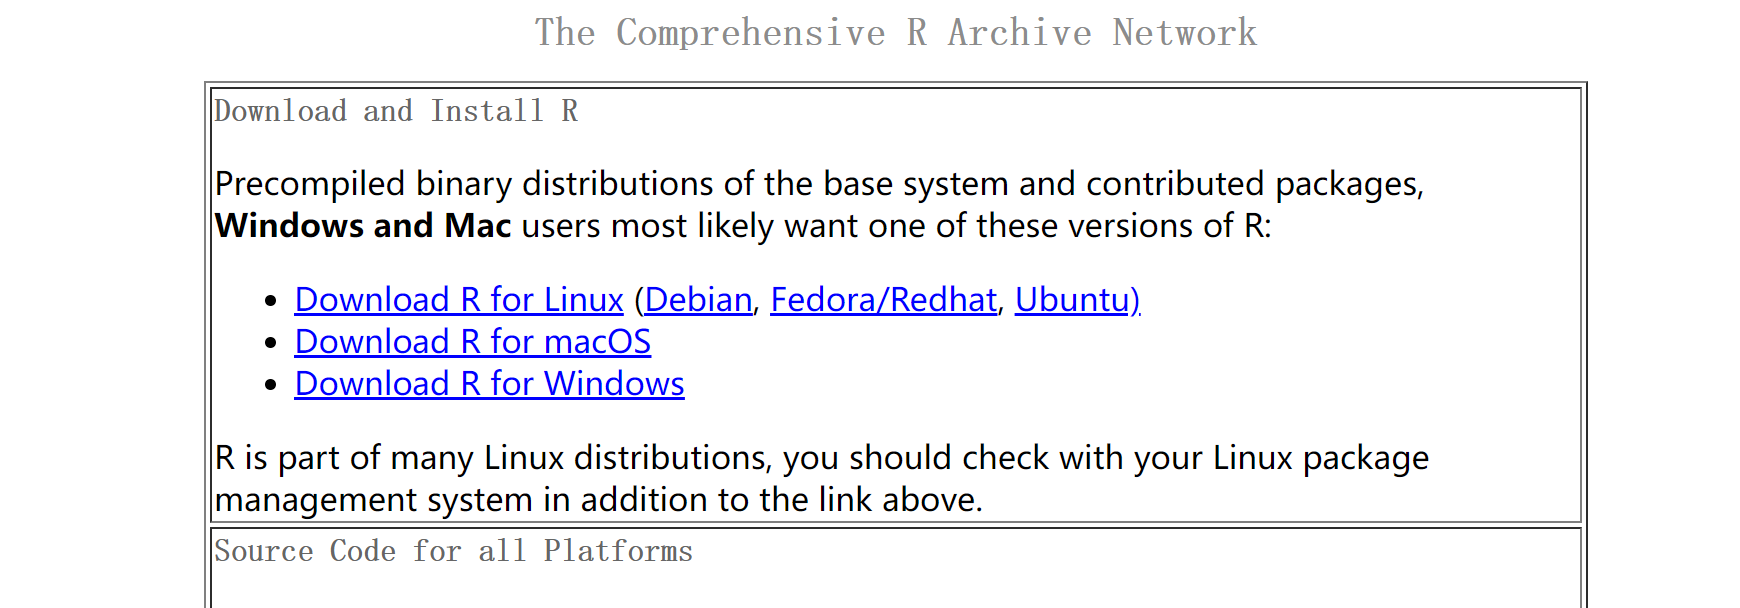
\includegraphics[width=\linewidth]{s3.PNG}
  \end{columns}
\end{frame}

\begin{frame}{Windows 与 macOS 的安装文件}
  \begin{columns}[T,onlytextwidth]
    \column{0.48\textwidth}
      \textbf{Windows}
      \begin{itemize}
        \item 进入 \textbf{Download R for Windows}
        \item 选择 \textbf{base}
        \item 下载当前稳定版的 \code{.exe} 文件
        \item 按安装向导完成安装
      \end{itemize}
    \column{0.48\textwidth}
      \textbf{macOS}
      \begin{itemize}
        \item 进入 \textbf{Download R for macOS}
        \item Apple 芯片选择 \code{arm64.pkg}
        \item 较早的 Intel 机型选择 \code{x86\_64.pkg}
        \item 打开 \code{.pkg} 文件完成安装
      \end{itemize}
  \end{columns}
  \vfill
  {\small Windows：\href{https://cran.r-project.org/bin/windows/base/}{\texttt{cran.r-project.org/bin/windows/base/}}\par
   macOS：\href{https://cran.r-project.org/bin/macosx/}{\texttt{cran.r-project.org/bin/macosx/}}}
\end{frame}

\begin{frame}{RStudio Desktop 的下载与安装}
  \begin{columns}[T,onlytextwidth]
    \column{0.56\textwidth}
      \begin{enumerate}
        \item 确认 R 已经安装完成。
        \item 打开 RStudio IDE 官方下载页面。
        \item 选择 Open Source 版本的 RStudio Desktop。
        \item 下载与操作系统匹配的安装文件并安装。
        \item 启动 RStudio，确认 Console 可以正常显示。
      \end{enumerate}
      \vspace{0.3em}
      {\small 下载页面：\href{https://docs.posit.co/ide/user/}{\texttt{docs.posit.co/ide/user/}}}
    \column{0.40\textwidth}
      \centering
      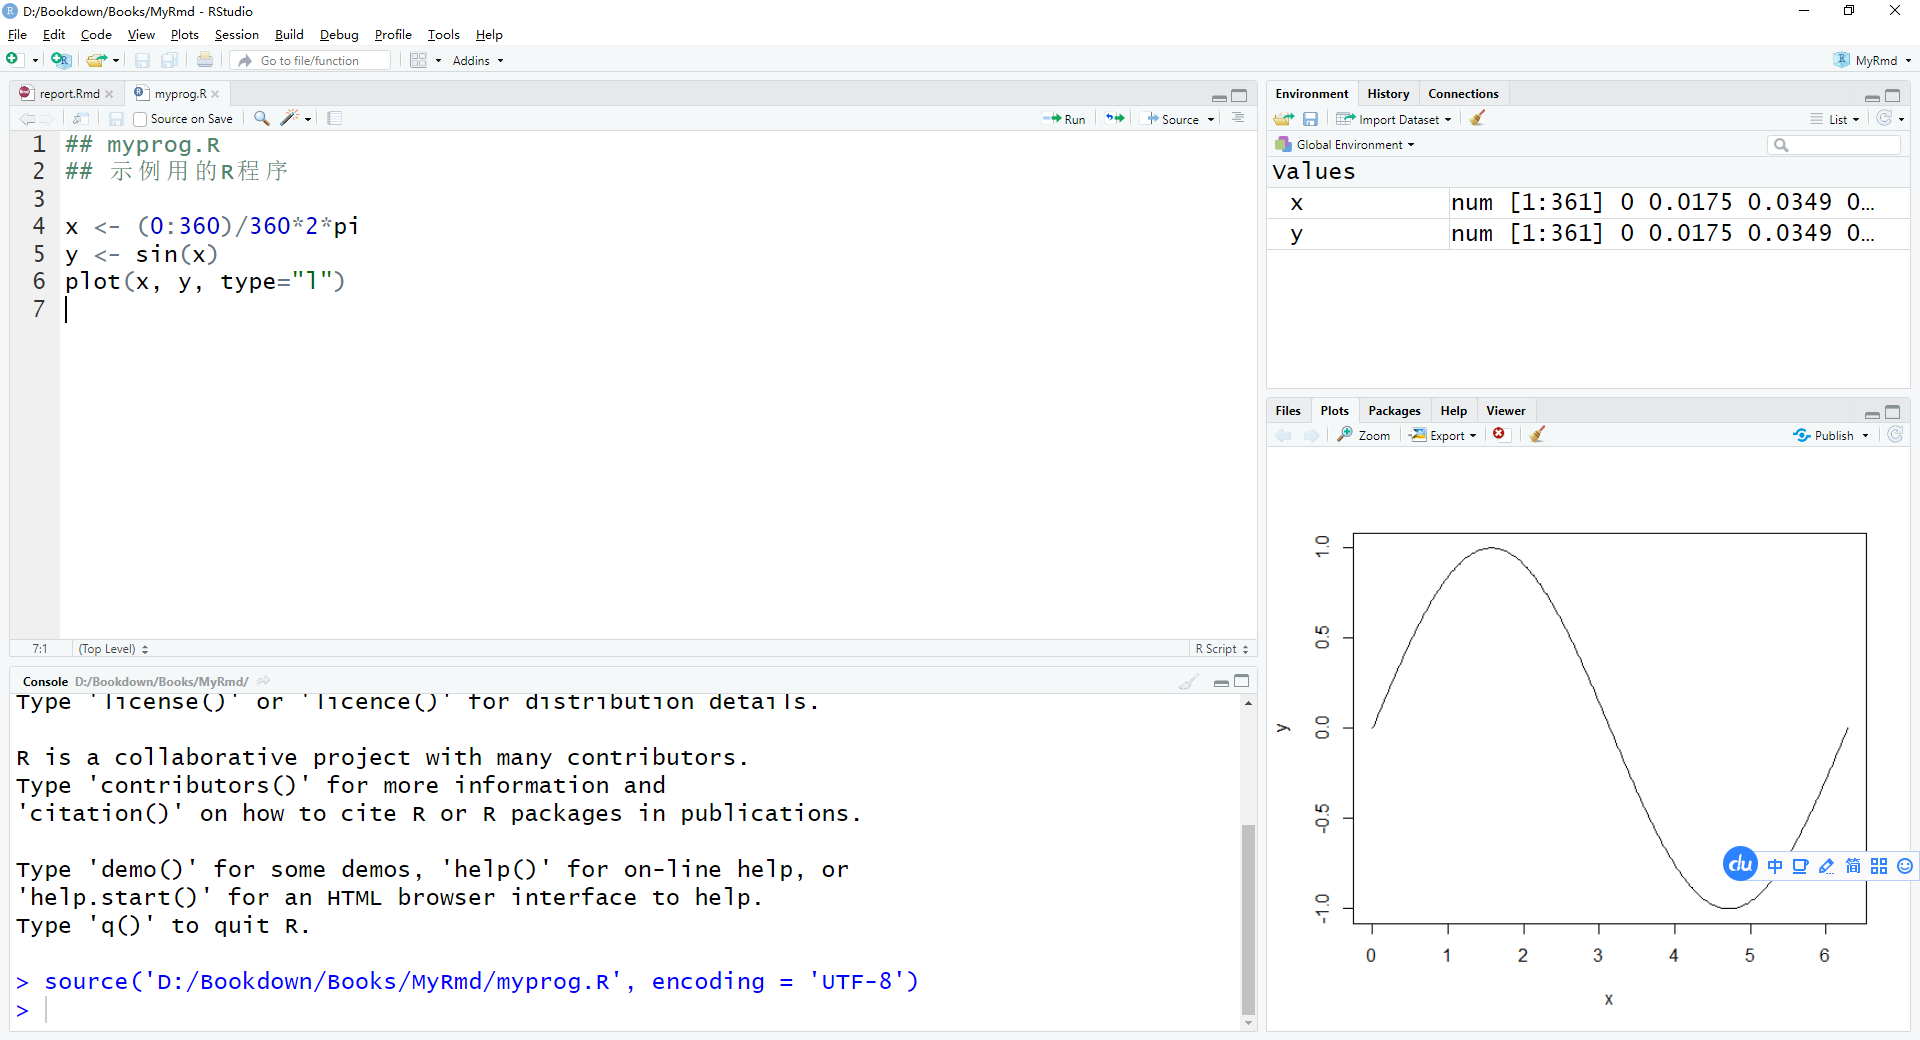
\includegraphics[width=\linewidth]{rstudio.png}
  \end{columns}
\end{frame}

\begin{frame}[fragile]{安装结果的验证}
  打开 RStudio，在 Console 中依次运行：
\begin{lstlisting}
R.version.string
1 + 1
\end{lstlisting}
  正常情况下，Console 会显示 R 的版本信息和计算结果：
\begin{lstlisting}
## [1] "R version ..."
## [1] 2
\end{lstlisting}
  如果 RStudio 无法启动或 Console 未加载 R，应先检查 R 是否已经正确安装，再检查 RStudio 版本是否与操作系统兼容。
\end{frame}

\begin{frame}{RStudio 的主要工作区}
  \begin{columns}[T,onlytextwidth]
    \column{0.58\textwidth}
      \centering
      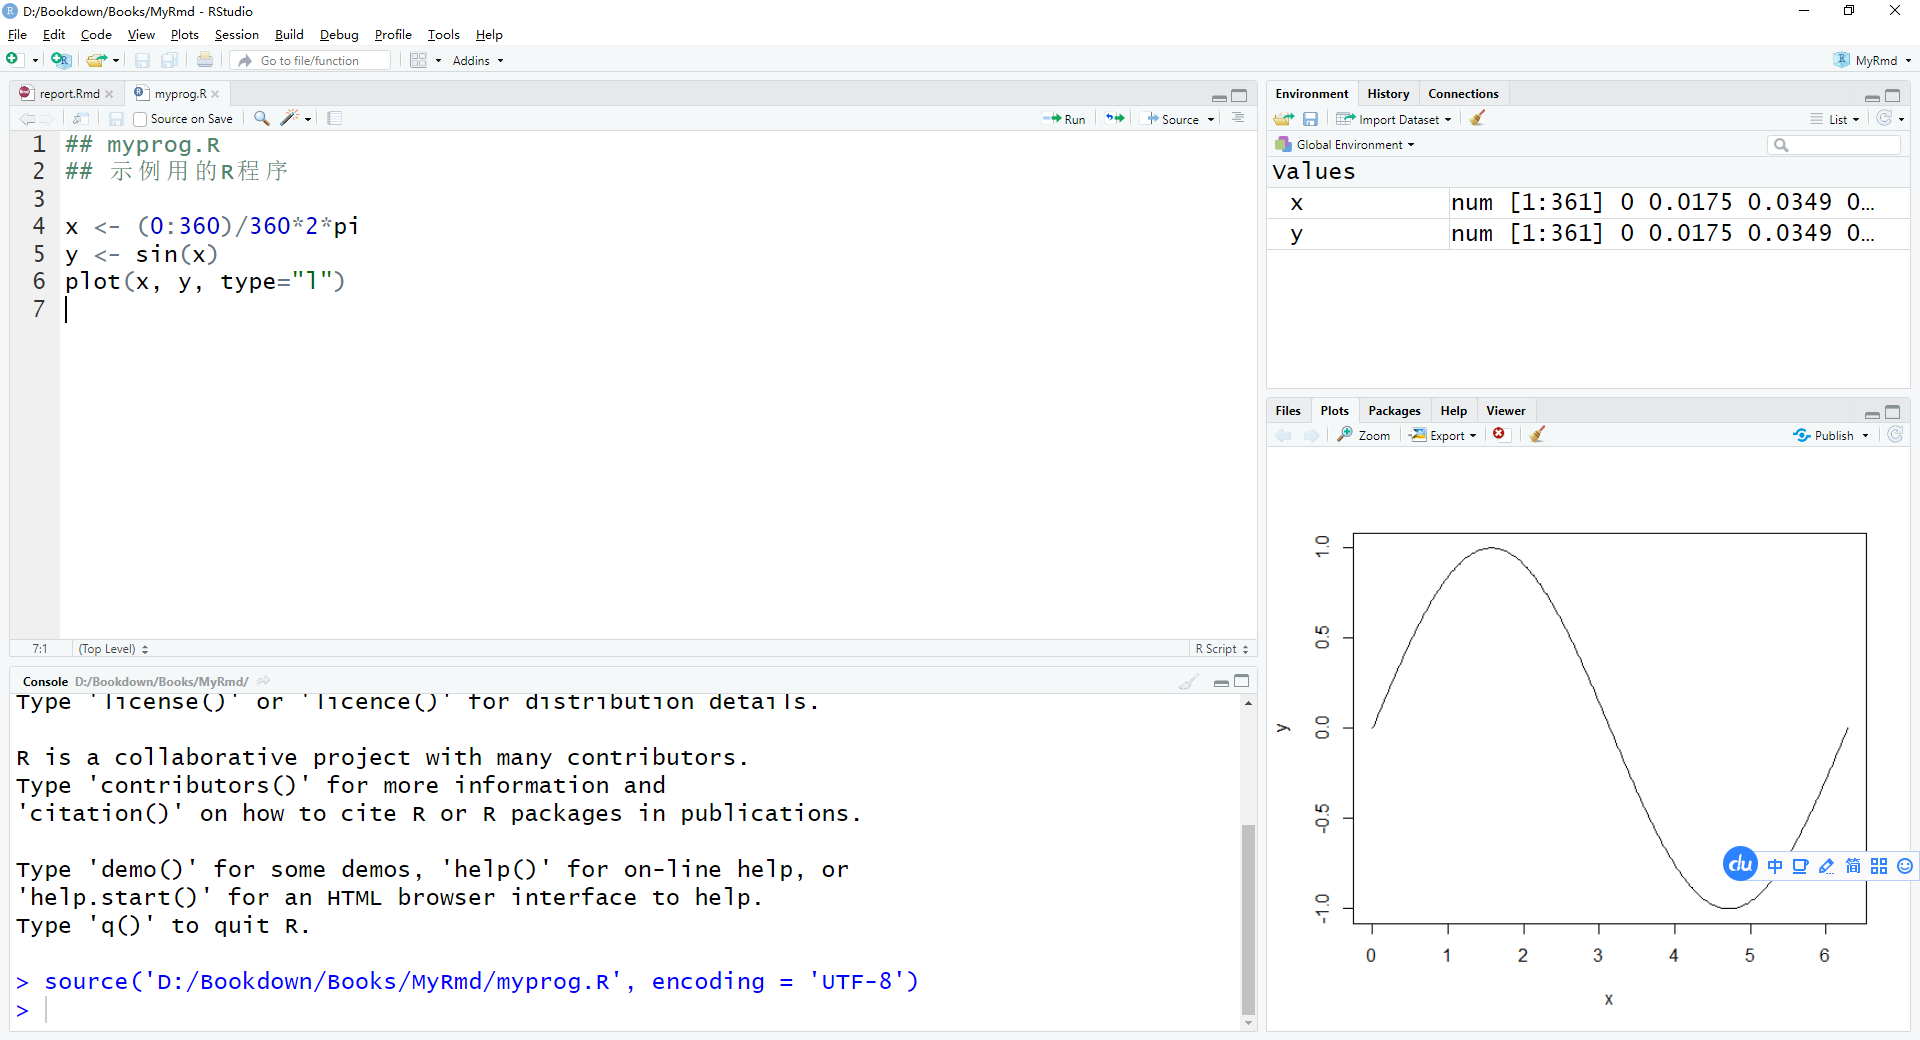
\includegraphics[width=\linewidth]{rstudio.png}
    \column{0.38\textwidth}
      \begin{enumerate}
        \item Source：编写脚本
        \item Console：显示运行结果
        \item Environment：查看对象
        \item Files / Plots / Help：管理文件、图形和帮助
      \end{enumerate}
  \end{columns}
\end{frame}

\begin{frame}{R 脚本的创建与运行}
  \begin{enumerate}
    \item 点击 \code{File > New File > R Script}。
    \item 立即保存，文件名设为 \code{R1-practice.R}。
    \item 本讲代码统一保存在该脚本中。
    \item Windows 使用 \code{Ctrl + Enter} 运行当前行；macOS 使用 \code{Command + Enter}。
    \item 也可以选中代码后点击 \code{Run}；Console 中输入的命令按 Enter 立即运行。
  \end{enumerate}
  \vspace{0.7em}
  \begin{block}{脚本与控制台}
    Console 显示即时结果；脚本保存完整代码，便于修改、复查和重复运行。
  \end{block}
\end{frame}

\begin{frame}[fragile]{脚本的基本结构}
  一个简短的分析脚本通常依次记录数据、计算过程和输出结果。
\begin{lstlisting}
# Data
day1 <- 35
day2 <- 45

# Analysis
average_time <- (day1 + day2) / 2

# Result
average_time
\end{lstlisting}
\end{frame}

\begin{frame}[fragile]{基本运算}
  在脚本中输入并逐行运行：
\begin{lstlisting}
1 + 1
5 * 8
100 / 4
2^3
\end{lstlisting}
  \begin{itemize}
    \item \code{*} 表示乘法，\code{/} 表示除法，\code{\^{}} 表示乘方。
    \item 圆括号可以改变运算顺序，例如 \code{(2 + 3) * 4}。
    \item R 按通常的数学规则确定运算顺序。
  \end{itemize}
\end{frame}

\begin{frame}[fragile]{注释与输出}
\begin{lstlisting}
# average reading time for two days
(35 + 45) / 2
## [1] 40
\end{lstlisting}
  \begin{itemize}
    \item 井号 \code{\#} 后面的文字是注释，R 不会执行它。
    \item \code{[1]} 是输出位置的提示，不是答案的一部分。
    \item 注释用于记录分析目的、数据来源和处理依据。
  \end{itemize}
  \vspace{0.4em}
  不写与代码内容重复的注释，优先记录必要的背景信息。
\end{frame}

\begin{frame}[fragile]{对象与赋值}
\begin{lstlisting}
day1 <- 35
day2 <- 45
average_time <- (day1 + day2) / 2
average_time
## [1] 40
\end{lstlisting}
  \begin{itemize}
    \item \code{<-} 是赋值运算符，将右侧的值赋给左侧对象。
    \item 对象名应反映数据含义，并注意 R 区分大小写。
    \item 赋值语句运行后，Environment 中将显示相应对象。
  \end{itemize}
\end{frame}

\begin{frame}[fragile]{函数与参数}
  函数接收输入并返回结果，圆括号中填写函数所需的参数。
\begin{lstlisting}
sqrt(25)
round(3.14159, digits = 2)
mean(c(35, 45))

?mean
\end{lstlisting}
  \begin{itemize}
    \item \code{sqrt()}、\code{round()} 和 \code{mean()} 是函数。
    \item \code{digits = 2} 指定保留两位小数。
    \item \code{?mean} 打开函数帮助；\code{help.start()} 打开帮助系统；\href{https://www.rdocumentation.org/}{RDocumentation} 可检索函数及扩展包文档。
  \end{itemize}
\end{frame}

\begin{frame}[fragile]{向量的创建}
  向量是由相同基本类型元素构成的一维数据结构。
\begin{lstlisting}
reading_time <- c(25, 40, 35, 50, 20,
                  45, 30, 55, 40, 60)

reading_time
\end{lstlisting}
  \begin{itemize}
    \item \code{c()} 将多个元素组合为一个向量。
    \item 函数参数之间使用逗号分隔。
    \item 对象名 \code{reading\_time} 表明该向量记录阅读时间。
  \end{itemize}
\end{frame}

\begin{frame}[fragile]{向量化计算}
  对向量进行运算时，R 会对其中每个元素执行相同的计算。
\begin{lstlisting}
reading_hours <- reading_time / 60
round(reading_hours, digits = 2)

## [1] 0.42 0.67 0.58 0.83 0.33
## [6] 0.75 0.50 0.92 0.67 1.00
\end{lstlisting}
  上述代码把每条阅读时间记录从分钟转换为小时。与逐个计算相比，向量化写法更简洁，也便于复查。
\end{frame}

\begin{frame}[fragile]{基本汇总函数}
\begin{lstlisting}
sum(reading_time)
length(reading_time)
mean(reading_time)

## [1] 400
## [1] 10
## [1] 40
\end{lstlisting}
  \begin{block}{统计解释}
    在本例给出的 10 条记录中，平均阅读时间为 40 分钟。该结果仅描述现有观测，不涉及对其他学生或其他日期的总体推断。
  \end{block}
\end{frame}

\begin{frame}[fragile]{课堂练习一：向量与汇总函数}
  某项调查记录了八名学生一天内的阅读页数：
\begin{lstlisting}
pages <- c(18, 25, 20, 30, 22, 27, 24, 34)
\end{lstlisting}
  完成以下计算：
  \begin{enumerate}
    \item 用 \code{length()} 查看记录数。
    \item 用 \code{sum()} 计算总页数。
    \item 用 \code{mean()} 计算平均页数。
    \item 根据数据背景表述平均数的含义。
  \end{enumerate}
  \vfill
  \hfill 建议时间：6 分钟
\end{frame}

\begin{frame}[fragile]{课堂练习一：结果核对}
\begin{lstlisting}
length(pages)
sum(pages)
mean(pages)

## [1] 8
## [1] 200
## [1] 25
  \end{lstlisting}
  \begin{block}{结果表述}
    八名学生一天阅读页数的平均值为 25 页。平均数概括观测值的整体水平，不意味着每名学生均阅读 25 页。
  \end{block}
\end{frame}

\begin{frame}[fragile]{缺失值的识别与处理}
\begin{lstlisting}
ratings <- c(4, 5, 3, 4, 5, 2, 4, NA, 3, 5)

mean(ratings)
## [1] NA

mean(ratings, na.rm = TRUE)
## [1] 3.888889
\end{lstlisting}
  \begin{itemize}
    \item \code{NA} 表示该位置的观测值缺失。
    \item \code{na.rm = TRUE} 表示本次计算排除缺失观测。
    \item 报告结果时应说明缺失值数量及其处理方式。
  \end{itemize}
\end{frame}

\begin{frame}[fragile]{常见错误信息及排查}
  \small
  \renewcommand{\arraystretch}{0.92}
  \begin{tabular}{p{0.34\textwidth}p{0.58\textwidth}}
    \toprule
    \textbf{错误信息或现象} & \textbf{检查内容} \\
    \midrule
    \code{object not found} & 是否运行了赋值语句；大小写是否一致 \\
    \code{unexpected symbol} & 逗号、括号或引号是否遗漏 \\
    Console 出现 \code{+} & 上一行可能没有结束；按 Esc 后检查 \\
    得到 \code{NA} & 数据中是否存在缺失值 \\
    \bottomrule
  \end{tabular}
  \vspace{0.6em}

  排查顺序：错误信息、代码位置、语法结构、对象状态。
\end{frame}

\begin{frame}[fragile]{课堂练习二：缺失值与描述性汇总}
  某项调查记录了 10 位读者对一篇作品的评分：
\begin{lstlisting}
ratings <- c(4, 5, 3, 4, 5, 2, 4, NA, 3, 5)
\end{lstlisting}
  完成以下分析：
  \begin{enumerate}
    \item 查看向量长度，并计算有效评分的数量。
    \item 计算有效评分的平均数。
    \item 找出最低分和最高分：\code{min()}、\code{max()}。
    \item 计算评分的极差：最高分减最低分。
    \item 表述分析结果，并说明缺失值的处理方式。
  \end{enumerate}
  \vfill
  \hfill 建议时间：12 分钟
\end{frame}

\begin{frame}[fragile]{课堂练习二：参考结果}
\begin{lstlisting}
length(ratings)
sum(!is.na(ratings))
mean(ratings, na.rm = TRUE)
min(ratings, na.rm = TRUE)
max(ratings, na.rm = TRUE)
max(ratings, na.rm = TRUE) - min(ratings, na.rm = TRUE)
\end{lstlisting}
  \begin{block}{结果表述}
    10 条记录中有 9 个有效评分。有效评分的平均值约为 3.89，最低值为 2，最高值为 5，极差为 3；计算时排除了 1 个缺失观测。
  \end{block}
\end{frame}

\begin{frame}{本讲小结}
  \begin{itemize}
    \item R 负责统计计算，RStudio 提供代码编辑和结果管理环境。
    \item 脚本应保存数据、计算过程和必要的注释。
    \item \code{<-} 用于赋值，\code{c()} 用于创建向量，函数用于完成计算。
    \item 汇总数据时应检查缺失值，并在结果解释中说明处理方式。
    \item 出现错误时，先阅读 Console 信息并定位刚刚运行的代码。
  \end{itemize}
  \vfill
  \centering 本讲不布置课后作业。
\end{frame}

\appendix

\begin{frame}[fragile]{补充：科学记数法与复合表达式}
\begin{lstlisting}
5 + (2.3 - 1.125) * 3.2 / 1.1 + 1.23E3
## [1] 1238.418
\end{lstlisting}
  \begin{itemize}
    \item \code{1.23E3} 表示 $1.23\times 10^3$。
    \item R 按括号、乘方、乘除、加减的顺序计算表达式。
    \item 乘法使用 \code{*}，除法使用 \code{/}，乘方使用 \code{\^{}}。
    \item 输入代码时应使用英文标点，避免中文逗号和引号造成语法错误。
  \end{itemize}
\end{frame}

\begin{frame}[fragile]{补充：常用数学函数}
\begin{lstlisting}
sqrt(6.25)       # 2.5
exp(1)           # 2.718282
log10(10000)     # 4

round(1.1234, 2) # 1.12
floor(1.1234)    # 1
ceiling(1.1234)  # 2
\end{lstlisting}
  \begin{itemize}
    \item \code{sqrt()}、\code{exp()} 和 \code{log10()} 分别计算平方根、自然指数和常用对数。
    \item \code{round()}、\code{floor()} 和 \code{ceiling()} 分别用于四舍五入、向下取整和向上取整。
  \end{itemize}
\end{frame}

\begin{frame}[fragile]{补充：圆周率与三角函数}
\begin{lstlisting}
pi
## [1] 3.141593
sin(pi / 6)
## [1] 0.5
cos(pi / 6)
## [1] 0.8660254
tan(pi / 6)
## [1] 0.5773503
\end{lstlisting}
  R 的三角函数以弧度为单位。\code{pi} 是 R 内置的圆周率常量。
\end{frame}

\begin{frame}[fragile]{补充：常量与基本类型}
  常量是直接写在代码中的值。R 中常见的常量包括：
  \begin{itemize}
    \item 数值型：\code{123}、\code{123.45}
    \item 字符型：\code{"Li Ming"}、\code{'Li Ming'}
    \item 逻辑型：\code{TRUE}、\code{FALSE}
    \item 缺失值：\code{NA}
  \end{itemize}
  \vspace{0.5em}
  同一向量通常用于保存相同基本类型的数据。字符型常量必须置于英文单引号或双引号中。
\end{frame}

\begin{frame}[fragile]{补充：特殊数值}
  \begin{itemize}
    \item \code{NA} 表示缺失的观测值。
    \item \code{NaN} 表示无法定义的数值结果，例如 \code{0 / 0}。
    \item \code{Inf} 和 \code{-Inf} 表示正无穷和负无穷，例如 \code{1 / 0}。
  \end{itemize}
\begin{lstlisting}
0 / 0
## [1] NaN
1 / 0
## [1] Inf
\end{lstlisting}
  \code{NA}、\code{NaN} 和 \code{Inf} 的含义不同，数据检查时应分别识别。
\end{frame}

\begin{frame}[fragile]{补充：对象命名与赋值}
  \begin{itemize}
    \item 对象名可以包含字母、数字、下划线和句点，但不能以数字开头。
    \item R 区分大小写，\code{y} 与 \code{Y} 是两个不同的对象。
    \item 对象可以保存数值、向量、矩阵、数据框和函数等内容。
    \item \code{<-} 和 \code{=} 均可用于赋值；本课程统一使用 \code{<-}。
  \end{itemize}
\begin{lstlisting}
x <- 10
x1 <- 20
cancer.tab <- c(3, 5, 8)
\end{lstlisting}
\end{frame}

\end{document}
